\chapter{Návrh aplikácie}

Pri vývoji aplikácie budem používať všetky technológie spomenuté v \emph{Technológie strany klienta}. Keďže tieto technológie na vývoj webovej aplikácie nestačia musím si zvoliť technológiu, ktorú použijem na strane servera. Rozhodol som sa zvoliť si jazyk Ruby, pretože už mám s ním niekoľko rokov skúseností, a dokážem v ňom tvoriť webové aplikácie rýchlo a efektívne.

\section{Jazyk -- Ruby}

Ruby je dynamický, reflektívny objektovo orientovaný programovací jazyk, ktorý kombinuje syntax inšpirovanú jazykmi Perl, Smalltalk, Eiffel, Lisp a má dynamickú správu pamäti. Autor -- Yukihiro Matsumoto -- pri návrhu vychádzal z filozofie, že programátor by sa pri práci s jazykom mal baviť ale zároveň byť produktívny. Taktiež zdôrazňoval, že dizajn systémov by sa mal zameriavať viac na potreby človeka ako na potreby počítača. \citep{matsumoto2002ruby}

\subsection{Zaujímavé vlastnosti jazyka Ruby}

Ruby je veľmi zaujímavý jazyk, avšak má mnoho vlastností, ktoré by mohli samostatne pokryť ďalšiu prácu. Preto som sa rozhodol vybrať také, ktoré sú netradičné pre iné programovacie jazyky a priblížiť ich.

\clearpage
\subsubsection{Premenné}

Ruby často používa veľmi obmedzenú interpunkciu, ale niektoré znaky sú použité na dekoráciu. Ďalšia vlastnosť je, že Ruby nepotrebuje deklarovať premenné. Zároveň sa používajú jednoduché konvencie na odlíšenie rozsahu premenných:

\begin{itemize}
    \item \emph{var} je lokálna premenná
    \item \emph{@var} je premenná inštancie triedy
    \item \emph{@@var} je premenná triedy
    \item \emph{\texttt{\$var}} je globálna premenná
\end{itemize}

Tieto znaky uľahčujú čitateľnosť výsledného kódu a umožňujú programátorovi jednoducho rozoznať roly každej premennej. \citep{web:rubylang}

\subsubsection{Funkcie - zátvorky nepotrebné }

Funkcie v Ruby sú zaujímavé z pohľadu, že pri volaní funkcie nemusíme napísať zátvorky funkcie, čiže tieto dve funkcie sú ekvivalentné:

\begin{minted}{ruby}
redirect_to(courses_path)
redirect_to courses_path
\end{minted}

Toto pravidlo platí do istej miery aj pre polia a hash-e, ale len pri ich zadávaní ako parametrov do funkcie. V niektorých prípadoch je však nutné presne vymedziť kde hash začína a končí inak môže vzniknúť problém, že sa funkcia s takým počtom parametrov sa nenájde.

\subsubsection{Symboly}

Symbol na prvý pohľad vyzerá ako premenná, ktorá má pred názvom dvojbodku, napríklad \emph{:user}. Výhodou symbolov je, že ich nie je potrebné deklarovať a v celom programe budú rovnaké. Zoberme nasledujúci príklad:

\begin{minted}{ruby}
puts "string".object_id
puts "string".object_id
puts :symbol.object_id
puts :symbol.object_id
\end{minted}

Po spustení tohto programu sa zobrazil nasledujúci výstup a naozaj dokázal, že symboly sú počas behu programu rovnaké:

\begin{minted}{bash}
$ ruby symbol.rb
90520360
90520080
801628
801628
\end{minted}

\subsubsection{Bloky}

Blok je v podstate časť programu vložená medzi \emph{do} a \emph{end}. Sú dva spôsoby ako napísať blok:

\begin{itemize}
    \item Viacriadkový, medzi \emph{do} a \emph{end}
    \item V jednom riadku, medzi \emph{\{} a \emph{\}}
\end{itemize}

\begin{minted}{ruby}
# Viac riadkový blok
[1, 2, 3].each do |n|
  puts "Cislo #{n}"
end

# Jednoriadkový blok
[1, 2, 3].each { |n| puts "Cislo #{n}" }
\end{minted}

Obe verzie tohto kódu vypíšu Cislo 1, Cislo 2 a Cislo 3 v poradí. Malé \emph{n}, ktoré vidíme medzi ``absolútnou hodnotou'' je \textbf{parameter bloku} a jeho hodnota v tomto prípade bude číslo v poradí ako sú uložené v poli. Čiže, pri prvej iterácii bude mať hodnotu 1, v ďalšej 2 a v poslednej 3.

\emph{Yield}, je ďalšie kľúčové slovo, ktoré dovoľuje funkciám použiť bloky priamo v tele. Funguje nasledujúco:

\begin{minted}{ruby}
def moja_funkcia
  puts "Zaciatok funkcie"
  yield
  puts "Koniec funkcie"
end

# Zavolanie funkcie spolu s blokom
moja_funkcia do
  puts "Funkcia je v yield-e"
end
\end{minted}

Po spustení programu vyššie dostaneme takýto výstup:
\begin{minted}{bash}
Zaciatok funkcie
Funkcia je v yield-e
Koniec funkcie
\end{minted}

Čiže, keď funkcia príde k \emph{yield}-u tak program definovaný v bloku funkcie sa spustí a po dokončení bloku funkcia pokračuje ďalej. 

Blok môžeme dodať akejkoľvek funkcii ale ak nemá v tele použitý \emph{yield} tak sa blok nespustí. Naopak, ak je \emph{yield} použitý ale nedodáme blok bude vyvolaná výnimka. Preto ak chceme spraviť dodanie bloku voliteľné musíme použiť \emph{\texttt{block\_given?}} a kontrolovať či bol block dodaný a až vtedy vyvolať \emph{yield}.

\clearpage
Každý parameter zadaný v \emph{yield} bude posunutý ako parameter bloku pri jeho použití presne v poradí v akom sú zadané do \emph{yield}:

\begin{minted}{ruby}
def moja_funkcia
  yield("Adam", 10)
end

moja_funkcia do |meno, vek| 
  puts "#{meno} má #{vek} rokov"
end
\end{minted}

\subsubsection{Moduly}

Ruby nepodporuje viacnásobnú dedičnosť. Keď teda chceme aby trieda implementovala určitú funkcionalitu, ale dedičnosť sme už využili, musíme využiť \emph{Module}. Module je kolekcia metód, konštánt a môžeme ho definovať nasledujúco:

\begin{minted}{ruby}
module Mod
  def moja_funkcia(arg)
    puts arg
  end
end
\end{minted}

V triede kde požadujeme funkcionalitu modulu potom jednoducho zahrnieme modul pomocou funkcie \emph{include()}. Napríklad:

\begin{minted}{ruby}
class MyClass < ParentClass
    include Mod
end
\end{minted}

\subsection{RubyGems}

RubyGems je správca balíčkov používaný spolu s jazykom Ruby, ktorý ponúka štandardný formát pre distribúciu Ruby programov a knižníc vo formáte nazývanom \emph{gem} a uľahčuje ich inštaláciu. Všetky balíčky sa dajú nájisť, prehľadávať alebo pridávať na stránke \url{https://rubygems.org}.

\section{Framework -- Ruby on Rails}

Ruby on Rails je framework pre tvorbu webových aplikácii na strane servera pomocou jazyka Ruby. Bol vytvorený v roku 2006 a jeho autorom je David Heinemeier Hansson. Framework je vytvorený na zaujímavej ideológii - konvencia má prednosť pred konfiguráciou. To znamená, že ak vývojár vytvára webovú aplikáciu s pomocou Ruby on Rails tak nastavuje len to čo je dôležité pre chod aplikácie.
Ak vývojár dodržuje tieto konvencie tak spraví menej rozhodnutí, čoho výsledkom je rýchlejší čas vývoja, vylepšená spolupráca na projekte a jednoduchšia údržba aplikácie.

\subsection{Model, view a controller}

Ruby on Rails je založený na návrhovom vzore Model-view-controller (v skratke MVC). Ako názov naznačuje tento vzor sa skladá z troch dôležitých komponentov, ktoré riadia správanie sa aplikácie.

\begin{itemize}
    \item \textbf{Model} reprezentuje iba dáta. Nie je závislý na controller-och alebo view-och
    \item \textbf{View} zobrazuje dáta modelov a odosiela interakciu používateľa cotroller-om
    \item \textbf{Controller} poskytuje dáta z modelu do view-u a spracováva interakciu užívateľa, pričom ontroller je závislý na modeloch a view-och
\end{itemize}

\subsection{Active Record}

Active Record je Object-relational mapping (ORM) knižnica, ktorú Ruby on Rails využíva pre všetky svoje modely. Pri načítaní modelu z databázy sú všetky dáta uložené v pamäti, kde ich môžeme modifikovať a keď sa neskôr rozhodneme ich uložiť, tak Active Record odošle databáze SQL dotaz na zmenu týchto údajov.

\subsection{Migrácie}

Migrácie sú dôležitá súčasť knižnice Active Record, ktoré umožňujú aby sa schéma databázy menila priebežne. Obrovskou výhodou je, že zmeny v schéme sa nemenia pomocou čistého SQL, ale pomocou čistého Ruby DSL na popísanie zmien v tabuľkách.
Každá migrácia je uložená vo svojom súbore. Môže vyzerať napríklad takto:

\begin{minted}{ruby}
class CreateProducts < ActiveRecord::Migration[5.0]
  def change
    create_table :products do |t|
      t.string :name
      t.text :description
 
      t.timestamps
    end
  end
end
\end{minted}

Môžeme uvažovať, že každá migrácia je nová verzia schémy pre databázu. Schému môžeme napísať ručne alebo vygenerovať a potom doplniť operácie ktoré chceme vykonať ako pridanie/vymazanie tabuliek, stĺpcov, indexov alebo iných obmedzení.

\subsection*{Generátory súborov}

Ruby on Rails je nainštalovaný aj spolu s jednoduchou aplikáciou, ktorá nám okrem iných nástrojov pri vývoji umožňuje aj generovať súbory, čo nám značne uľahčuje a urýchľuje vývoj aplikácie. Generovanie z príkazového riadku prebieha naslednovne:

\begin{minted}{bash}
$ rails generate GENERATOR [args] [options]
\end{minted}

Slovo \emph{GENERATOR} zameníme za generátor, podľa toho aký súbor/y chceme vygenerovať. Ak do príkazového riadku zadáme iba \emph{rails generate} zobrazí sa nám krátka nápoveda ako generátory používať ale aj zoznam dostupných generátorov. Najdoležitejšie generátory pri vývoji aplikácie sú tieto:

\begin{itemize}
  \item controller
  \item mailer
  \item migration
  \item model
  \item task
\end{itemize}

Ďalej môžeme zadať argumenty, ktoré slúžia na vygenerovanie funkcií, stĺpcov alebo atribútov v závislosti od toho aký generátor máme zvolený.



\clearpage
\section{Databáza a entitno-relačný diagram}

\begin{figure}[!htb]
  \centering
  \hspace*{-0.5cm}
  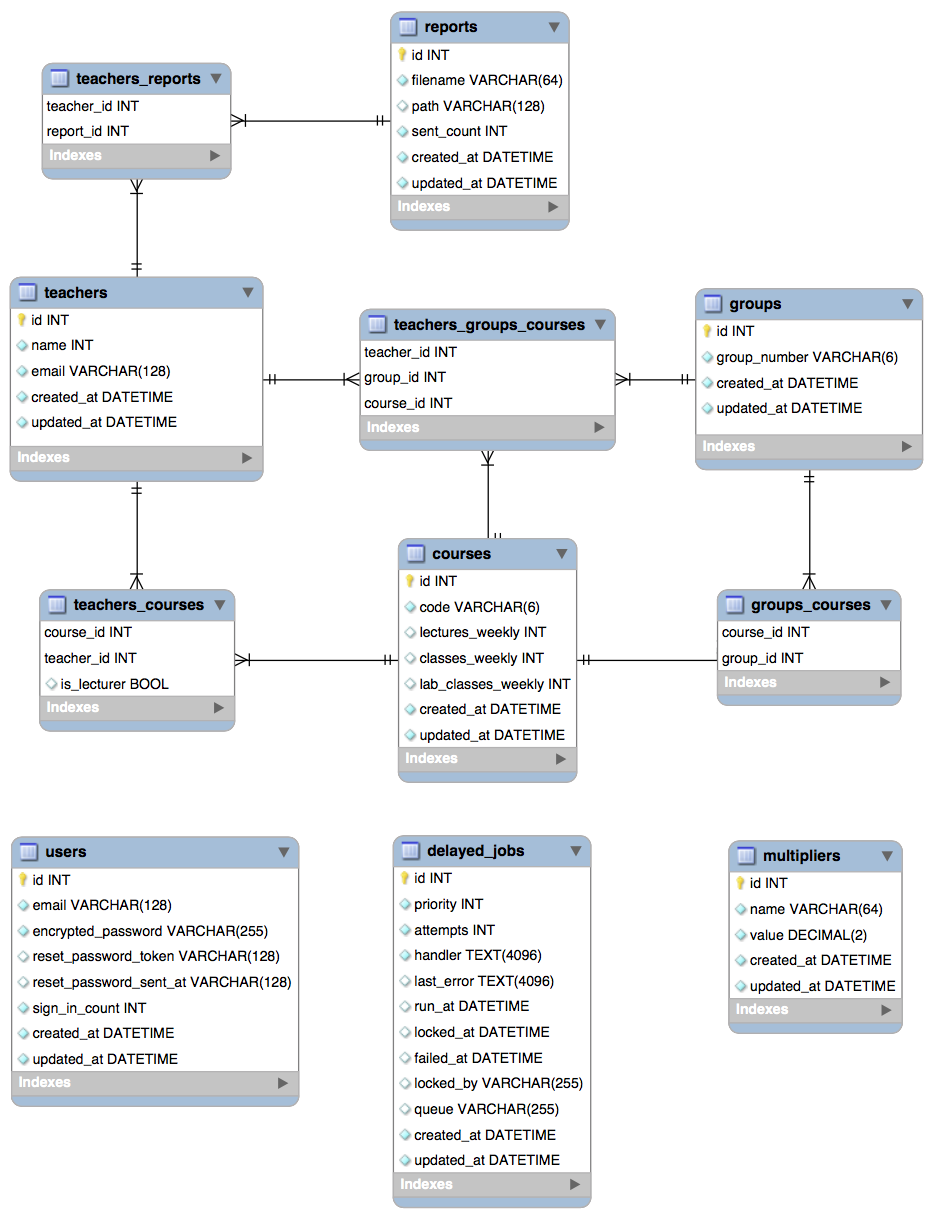
\includegraphics[width=0.9\textwidth]{content/images/db}
  \caption{Entitno-relačný diagram.}
\end{figure}

\clearpage
Diagram popisuje ako vyzerá výsledná verzia schémy databázy.

Na perzistentné uloženie dát aplikácie som zvolil databázu SQLite, ktorá má podľa mňa dostatočnú kapacitu a spĺňa všetky požiadavky pre škálu budovanej aplikácie. Má dokonca aj niekoľko výhod:

\begin{itemize}
    \item Jednoduchá inštalácia
    \item Nie je potrebná skoro žiadna konfigurácia
    \item Dáta sú ľahko zálohovateľné, pretože databáza je uložená v jedinom súbore
    \item Šetrí zdroje systému
\end{itemize}

\section{Systém pre správu verzií -- Git}

Pri tvorbe softvéru vývojári vytvárajú zdrojový kód. Menia, rozširujú ho, potrebujú vrátiť zmeny alebo sa vrátiť späť k starším verziám. Taktiež je potrebné zabezpečiť situáciu, keď na jednom projekte pracuje viac vývojárov naraz. \citep{otte2009version} 

Git je jedným z mnohých programov na správu verzií zdrojového kódu vytvorený Linusom Torvaldom v roku 2005. Používať ho budem počas celého vývoja aplikácie aj napriek tomu, že nie som súčasťou žiadneho týmu, pretože mi stále poskytuje niekoľko obrovských výhod, a to: 

\begin{itemize}
    \item Jednoduché a prehľadné zdieľanie zdrojového kódu s vedúcim práce
    \item História všetkých zmien zdrojového kódu
    \item Uľahčenie nasadenia na server
    \item Záloha aplikácie v prípade straty na lokálnom systéme
\end{itemize}

Existujú aj mnohé služby ktoré poskytujú hosting Git repozitárov či už platené, ako GitHub (\url{https://github.com/}) alebo open-source ako GitLab (\url{https://gitlab.com}), ktoré majú aj funkcionalitu zameranú na spoluprácu komunity ako \emph{Pull request} alebo sledovanie a nahlasovanie problémov, ktoré sa vyskytli pri používaní softvéru.